\section{Preliminaries}
\label{Sec:Preliminaries}
This section introduces the definitions and formalisms used in the paper. 
Logical formulas in our approach are defined over the theory of Linear Integer Arithmetic (LIA).
We use $X,X'$ to denote set of variables (unprimed and primed), where $X' = \{x'| x \in X\}$, $X$ is a set of state variables, and $X'$ is a set of next state variables.
If formula contains variables over multiple states, we use superscript notation, e.g., $X^{(0)}, \dots, X^{(n)}$ .

%

The formula defined over $X$ is a state formula, and a formula over $X \cup X'$ is a transition formula.
State formulas encode a set of states, and transition formulas define binary relations over the states.
Using $Id(X,X')$ we denote a transition formula $\bigwedge_{x \in X} x = x’$.

\textit{Transition systems and Safety Problem:} 
A \emph{transition system} (TS) is defined as $TS = \tuple{ Init, Tr, X }$, where $Init$ is a formula encoding the initial states of the system, $Tr$ is a transition formula, which encodes the transition relation, and $X$ is a set of system's variables.
With respect to transition system, a \emph{transition trace} is a formula encoding multiple consecutive transitions: $Tr^{n}(X^{(0)}, \dots, X^{(n)}) = Tr(X^{(0)}, X^{(1)}) \land \dots \land Tr(X^{(n-1)}, X^{(n)})$.
We write $Tr^{n}(X^{(0)},\dots,X^{(n)})$ for this conjunction throughout the paper.
A \emph{safety problem} is defined as  $P = \tuple{ Init, Tr, Bad, X }$ where $Bad$ is a formula representing states that violate the safety property.

%

Safety verification amounts to determining whether there exists a transition trace that reaches a $Bad$ state from the initial states.
If TS is safe, then there exists an inductive invariant $Inv(X)$ s.t. (1) $\forall X. Init(X) \rightarrow Inv(X)$, 
(2) $\forall X, X'. Inv(X) \land Tr(X,X') \rightarrow Inv(X')$, and (3) $\forall X. Inv(X) \rightarrow \lnot Bad(X)$.
We use \textsc{SafetyCheck}$(P)$ to denote a safety verification procedure that returns a tuple $\tuple{SAFE, Inv(X)}$ if 
TS is safe ($Inv(X)$ is inductive invariant).
% Otherwise, if TS is unsafe it returns $\tuple{UNSAFE, Tr^{n}(X^{(0)}, \dots, X^{(n)})}$, such that: 
If TS is unsafe it returns $\tuple{UNSAFE, Tr^{n}(X^{(0)}, \dots, X^{(n)})}$, where $\exists X^{(0)}, \dots, X^{(n)}.$

$$Init(X^{(0)}) \land Tr^{n}(X^{(0)}, \dots, X^{(n)}) \land Bad(X^{(n)})$$

\textit{Nontermination:}
A transition system is called \textbf{nonterminating} if there exists an initial state, from which it is possible to take 
any number of transitions, meaning $\exists X. Init(X)$ s.t.:
$$\forall n \in \mathbb{N}.  \exists X^{(1)}, \dots, X^{(n)}. Tr^{n}(X, X^{(1)}, \dots, X^{(n)})$$

\begin{definition}[Recurrent Set]
    For a Transition System $\tuple{ Init, Tr, X }$, a formula $N(X)$ is a recurrent set if: 
    (1) $\forall X. N(X) \rightarrow \exists X'. Tr(X,X') \land N(X')$,  
    (2) $\exists X. N(X) \land Init(X)$.
\end{definition}

Transition System is nonterminating if there exists a \emph{recurrent set}. 
Intuitively, every state in the recurrent set has a successor that also lies in the recurrent set, and the recurrent set contains some of the 
initial states.

\textit{Termination:} A TS is called \textbf{terminating} if for every initial state it is possible to take only limited number of transitions.
% For a Transition System $\tuple{ Init, Tr, X }$:
Transition System $\tuple{ Init, Tr, X }$ terminates, if $\forall X. Init(X)$ the following holds:
% $$\forall X. Init(X) \rightarrow \exists n \in \mathbb{N}. \lnot \exists \dots, X^{(n)}. Tr^{n}(X, X^{(1)}, \dots, X^{(n)})$$
$$\exists n \in \mathbb{N}. \lnot \exists X^{(1)}, \dots, X^{(n)}. Tr^{n}(X, X^{(1)}, \dots, X^{(n)})$$
% Termination can be proven by synthesizing a \emph{ranking function}~\cite{DBLP:conf/vmcai/PodelskiR04}, mapping states to a well-founded domain, such that its value strictly decreases along every transition.

\begin{definition}[Transition invariant]
    For a Transition System $\tuple{ Init, Tr, X }$, $\TrInv(X,X')$ is a transition invariant if: $\forall X,X'. R(X) \land Tr^+(X,X') \rightarrow \TrInv(X,X')$, where $Tr^+(X,X')$ is the transitive closure of $Tr(X,X')$
    and $R(X)$ is a formula encoding all the states, reachable within TS.
\end{definition}

\begin{definition}[Well-founded Relation]
    A binary relation $R \subseteq D \times D$ over a domain $D$ is \emph{well-founded} if there exists no infinite descending chain:
    $$\nexists\, d_0, d_1, d_2, \dots \in D.\ 
      \forall i \in \mathbb{N}.\ (d_i, d_{i+1}) \in R$$
\end{definition}

A relation $R(X,X')$ can be proven~\cite{DBLP:conf/vmcai/PodelskiR04} to be well-founded by synthesizing a ranking function $f(X)$, such that
 $\forall X,X'. R(X,X') \rightarrow f(X) > f(X')$.

\emph{Transition invariant}~\cite{DBLP:conf/lics/PodelskiR04} can be used to prove termination.
If transition invariant is a finite union of well-founded relations (for example if every separate relation has a ranking function), 
then the Transition System terminates.
\begin{definition}[Disjunctively well-founded relation]
    A relation $D(X,X') = \cup_{i = 0}^{n} R_i(X,X')$ is called disjunctively well-founded if every relation $R_i(X,X')$ is well-founded. 
\end{definition}

\textit{Craig Interpolation:} An abstraction technique~\cite{Craig_1957}, such that
given two formulas $A$ and $B$ where $A \land B$ is unsatisfiable, a Craig interpolant 
for $A$ and $B$ is a formula $I$. 
For $I$ the following holds: (1) $A \rightarrow I$; (2) $I \land B$ is unsatisfiable; 
and (3) $I$ only contains the symbols, common to both $A$ and $B$.
We use $Itp(A, B)$ to denote the computation of the Craig interpolant.

\subsection{Proving Nontermination via Safety}
Many techniques reduce termination and nontermination analysis to safety verification.
One notable approach is the reduction of nontermination to safety, which constructs
recurrent sets via inductive invariants~\cite{DBLP:conf/tacas/ChenCFNO14}.
It was introduced in the context of proving nontermination of programs with loops, and can be extended for the Transition Systems.
This approach is described below.

\begin{definition}[Sink states]
    For a Transition System $\tuple{Init, Tr, X }$, a state $s$ is a sink state, if $\lnot \exists s'. Tr(s,s')$.
    We use $\Sink(X)$ to denote the formula encoding all sink states in the transition system:
    $\forall X. \Sink(X) \leftrightarrow \lnot \exists X'. Tr(X,X')$
\end{definition}

\begin{figure}[t]
    \centering
    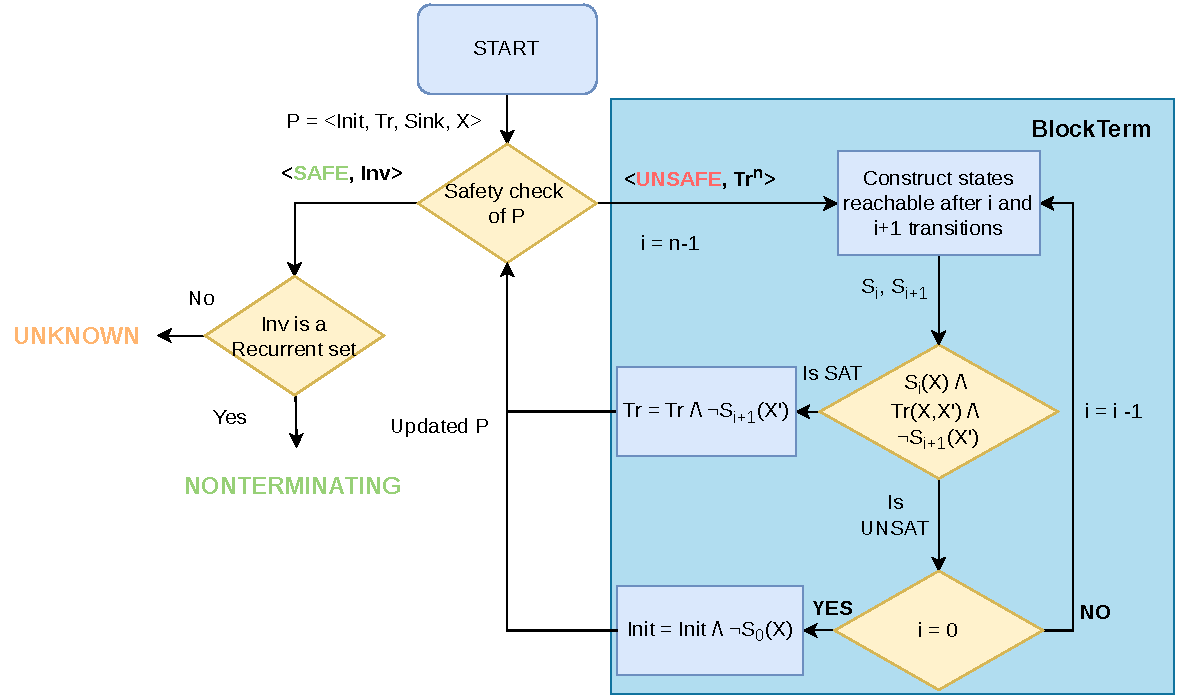
\includegraphics[width=\linewidth]{Figures/SNA.pdf}
    \caption{Execution flow of Safety-based Nontermination analysis, cf~\cite{DBLP:conf/tacas/ChenCFNO14}}
    \label{fig:SNA}
\end{figure}

Algorithm~\ref{Alg:SNA} for Safety-based Nontermination analysis (SNA) takes a 
safety problem $P = \tuple{Init, Tr, \Sink, X}$, where sink states are constructed from TS using
quantifier elimination, $\Sink(X) = \lnot QE(\exists X'. Tr(X,X'))$.
As an output, it returns \NONTERM{} if the system is nonterminating, and \UNKNOWN, if the algorithm cannot conclude the analysis. 
Figure~\ref{fig:SNA} contains the execution flow of Safety-based Nontermination.

\begin{algorithm}[t!]
	\SetInd{0.5em}{0.5em}
    \DontPrintSemicolon
    \small
    \newcommand{\Continue}{\textbf{continue}}
    \caption{Safety-based Nontermination Analysis (SNA), cf~\cite{DBLP:conf/tacas/ChenCFNO14}}
    \label{Alg:SNA}
    \SetKwInOut{Input}{Input}
    \SetKwInOut{Output}{Output}
    \Input{Safety problem $P = \tuple{\Init, \Tr, \Sink, X}$}
    \Output{\NONTERM $\mid$ \UNKNOWN}
    % \SetKwFunction{FAnalyze}{Analyze}
    % \SetKwProg{Fn}{Function}{:}{}
    % \nonl\Fn{\FAnalyze{$P$}}{
        \While{$\top$}{
            $\tuple{\res,\phi = Tr^{n}\ or \Inv} \gets \textsc{SafetyCheck}(P)$\\
            \label{SNA:UNSAFE}\eIf{$\res = \UNSAFE$} {
                $P \gets \blockTerm(P, \phi)$ \label{SNA:BLOCKTERM}
            }
            {
                \If{$\forall X. \phi(X) \rightarrow \exists X'. Tr(X,X')$\label{SNA:SAFE}}{
                    \Return \NONTERM \label{SNA:RECURRENT}
                }
                \Return \UNKNOWN
            }
            
        }
    % }
    
\end{algorithm}
% A

The approach executes a safety check of $P$ in a loop.
At line~\ref{SNA:UNSAFE}, the algorithm handles the case when $P$ is unsafe (i.e., exists a trace reaching sink states).
In this case, the algorithm calls the $\blockTerm$ procedure (Algorithm~\ref{Alg:SNABlock}), which refines the safety problem $P$ by blocking the states that deterministically
lead to the sink states, updating the Safety problem.
$\blockTerm$ is described in detail below.
In the case when $P$ is safe, the algorithm checks if the inductive invariant $Inv(X)$ is a recurrent set (line~\ref{SNA:SAFE}).
The check at line~\ref{SNA:SAFE} is executed using quantifier elimination, checking if the following formula
is unsatisfiable:
$$\exists X. \phi(X) \land \lnot QE(\exists X'. Tr(X,X')).$$
If $Inv(X)$ is a recurrent set, then the transition system is nonterminating.
Otherwise, the algorithm returns \UNKNOWN.

\begin{algorithm}
    \SetInd{0.5em}{0.5em}
    \DontPrintSemicolon
    \small
    \newcommand{\Continue}{\textbf{continue}}
    \caption{\blockTerm(P, $Tr^{n}$), cf~\cite{DBLP:conf/tacas/ChenCFNO14}}
    \label{Alg:SNABlock}
    \SetKwInOut{Input}{Input}
    \SetKwInOut{Output}{Output}
    \SetKwInOut{Data}{Data}
    \Input{Safety problem $P = \tuple{Init, Tr, \Sink, X}$, terminating trace $Tr^{n}(X^{(0)}, \dots, X^{(n)}) = Tr(X^{(0)}, X^{(1)}) \land \dots \land Tr(X^{(n-1)}, X^{(n)})$}
    \Output{Refined safety problem $P'$}
    \Data{$S_0,\dots,S_n$ - formulas which encode states within trace reachable in 0, ..., n transitions}

    % \SetKwFunction{FBlock}{BlockTerm}
    % \SetKwProg{Fn}{Function}{:}{}
    % \Fn{\FBlock{$P, trace$}}{
    \SetAlgoFuncName{BlockTerm}{autoref name}
        $i \gets n-1$ \\
        \While{$i > 0$}{
            $S_{i+1}(X) \gets QE(\exists X^{(0)},\dots, X^{(i)},  X^{(i+2)}, \dots, X^{(n)}.$ $Init(X^{(0)}) \land Tr^{n} \land \Sink(X^{(n)}))[X^{(i+1)} \mapsto X]$ \label{SNA:Si1}\\
            $S_{i}(X) \gets QE(\exists X^{(0)},\dots, X^{(i-1)},  X^{(i+1)}, \dots, X^{(n)}.$ $Init(X^{(0)}) \land Tr^{n} \land \Sink(X^{(n)}))[X^{(i)} \mapsto X]$ \label{SNA:Si}\\
            \If{SAT ? $S_i(X) \land Tr(X,X') \land \lnot S_{i+1}(X')$ \label{SNA:BLOCK}}{
                $Tr'(X,X') \gets Tr(X,X') \land \lnot S_{i+1}(X')$ \label{SNA:TRBLOCK}  \\
                \Return $\tuple{Init, Tr', \Sink, X}$
            }
            $i \gets i - 1$   
        }
        $Init'(X^{(0)}) \gets Init(X^{(0)}) \land \lnot QE(\exists X^{(1)}, \dots, X^{(n)}. Init(X^{(0)}) \land Tr^{n} \land \Sink(X^{(n)}))$  \label{SNA:BLOCKINIT} \\
        \Return $\tuple{Init', Tr, \Sink, X}$
    % }
\end{algorithm}

The $\blockTerm$ procedure takes as input a safety problem $P$ and a trace formula $Tr^{n}(X^{(0)}, \dots, X^{(n)})$ such 
that $Init(X^{(0)}) \land Tr^{n}(X^{(0)}, \dots, X^{(n)}) \land \Sink(X^{(n)})$ is satisfiable.
The algorithm iteratively analyses the transition trace starting from the last transition. 
% It checks if it is possible to take a transition that does not lead to the sink states, starting from the end of the trace.
Algorithm~\ref{Alg:SNABlock} constructs states that are reachable after $i$ and $i+1$ transitions from the initial states using quantifier 
elimination at lines~\ref{SNA:Si1},~\ref{SNA:Si}.
Then, at line~\ref{SNA:BLOCK} it checks if $S_i(X) \land Tr(X,X') \land \lnot S_{i+1}(X')$ is satisfiable, sending a query to the SMT solver.
This query checks if it is possible to reach some state that does not necessarily lead to the sink states.
If it is possible, then the algorithm blocks the states that deterministically lead to the sink states at line~\ref{SNA:TRBLOCK}.
Otherwise, if the trace is deterministic, \blockTerm blocks the subset of initial states that leads to sink (line~\ref{SNA:BLOCKINIT}).


\begin{lemma}\label{Lem:NONTERM}
    If Algorithm~\ref{Alg:SNA} returns NONTERM, then the transition system is nonterminating, cf~\cite{DBLP:conf/vmcai/PodelskiR04}.
\end{lemma}
\begin{example}\label{Ex:SNA}
    Consider a transition system $TS = \tuple{Init, Tr, X}$ with 
    $X = \{x\}$, $Init(X)   \triangleq \top$, and
    $Tr(X, X') \triangleq (x' = x - 1 \lor x' = x - 2) \land x \neq 0$.
    The sink states are $\Sink(x) \triangleq v = 0$, and the initial 
    safety problem is $P = \tuple{Init, Tr, \Sink, x}$.
    This TS is nonterminating, since $x$ can infinitely decrease.

    The execution of Algorithm~\ref{Alg:SNA} updates initial states
    and transition in two iterations of the algorithm, via \blockTerm\: 
    $Init(X) \;\gets\; x \neq 0$, and  $Tr(X, X') \;\gets\; Tr(X, X') \land x' \neq 0$.
    The safety check of the updated problem concludes SAFE,
    with $Inv(X) \triangleq x \neq 0$. 
    $Inv(X)$ is a recurrent set, and algorihtm returns \textsc{NONTERM}.

    \textit{Motivation for transition invariant-based termination analysis.} Consider a 
    small modification (replacing $x\neq0$ with $x>0$): $Tr(X, X') \triangleq 
    (x' = x - 1 \lor x' = x - 2) \land x > 0$. 
    This renders $TS$ terminating, since $x$ is strictly positive and decreases every step. 
    However, Algorithm~\ref{Alg:SNA} cannot detect termination by design, and 
    it would return \UNKNOWN. 

    Let us examine the execution of Algorithm~\ref{Alg:SNA} on this example.
    First, using \blockTerm, it blocks initial states that instantly terminate:
    $Init(X) \;\gets\; x > 0$.
    In the second iteration, \textsc{SafetyCheck}$(P)$ returns UNSAFE with a 
    trace $Tr^1(X^{(0)}, X^{(1)})$, detecting that $\exists X^{(0)}, X^{(1)}. 
    Init(X^{(0)}) \land Tr^1(X^{(0)}, X^{(1)}) \land \lnot \Sink(X^{(1)})$.
    Our key insight is to generalise such traces into a formula, describing an 
    entire class of terminating behaviours. 
    If this generalisation yields a disjunctively well-founded 
    transition invariant over all reachable states, it witnesses 
    termination.
    Particularly, $\TrInv(X, X') \triangleq x' < x \land x > 0$ is a well-founded transition 
    invariant which proves the termination of $TS$.
    Section~\ref{sec:Main} presents the algorithm that automates this generalisation via 
    Craig interpolation.
\end{example}